\documentclass[tikz,border=8pt]{standalone}
\usepackage[utf8]{inputenc}
\usepackage[T1]{fontenc}
\usepackage{tikz}
\usetikzlibrary{arrows.meta,positioning,calc,decorations.pathreplacing}

\begin{document}
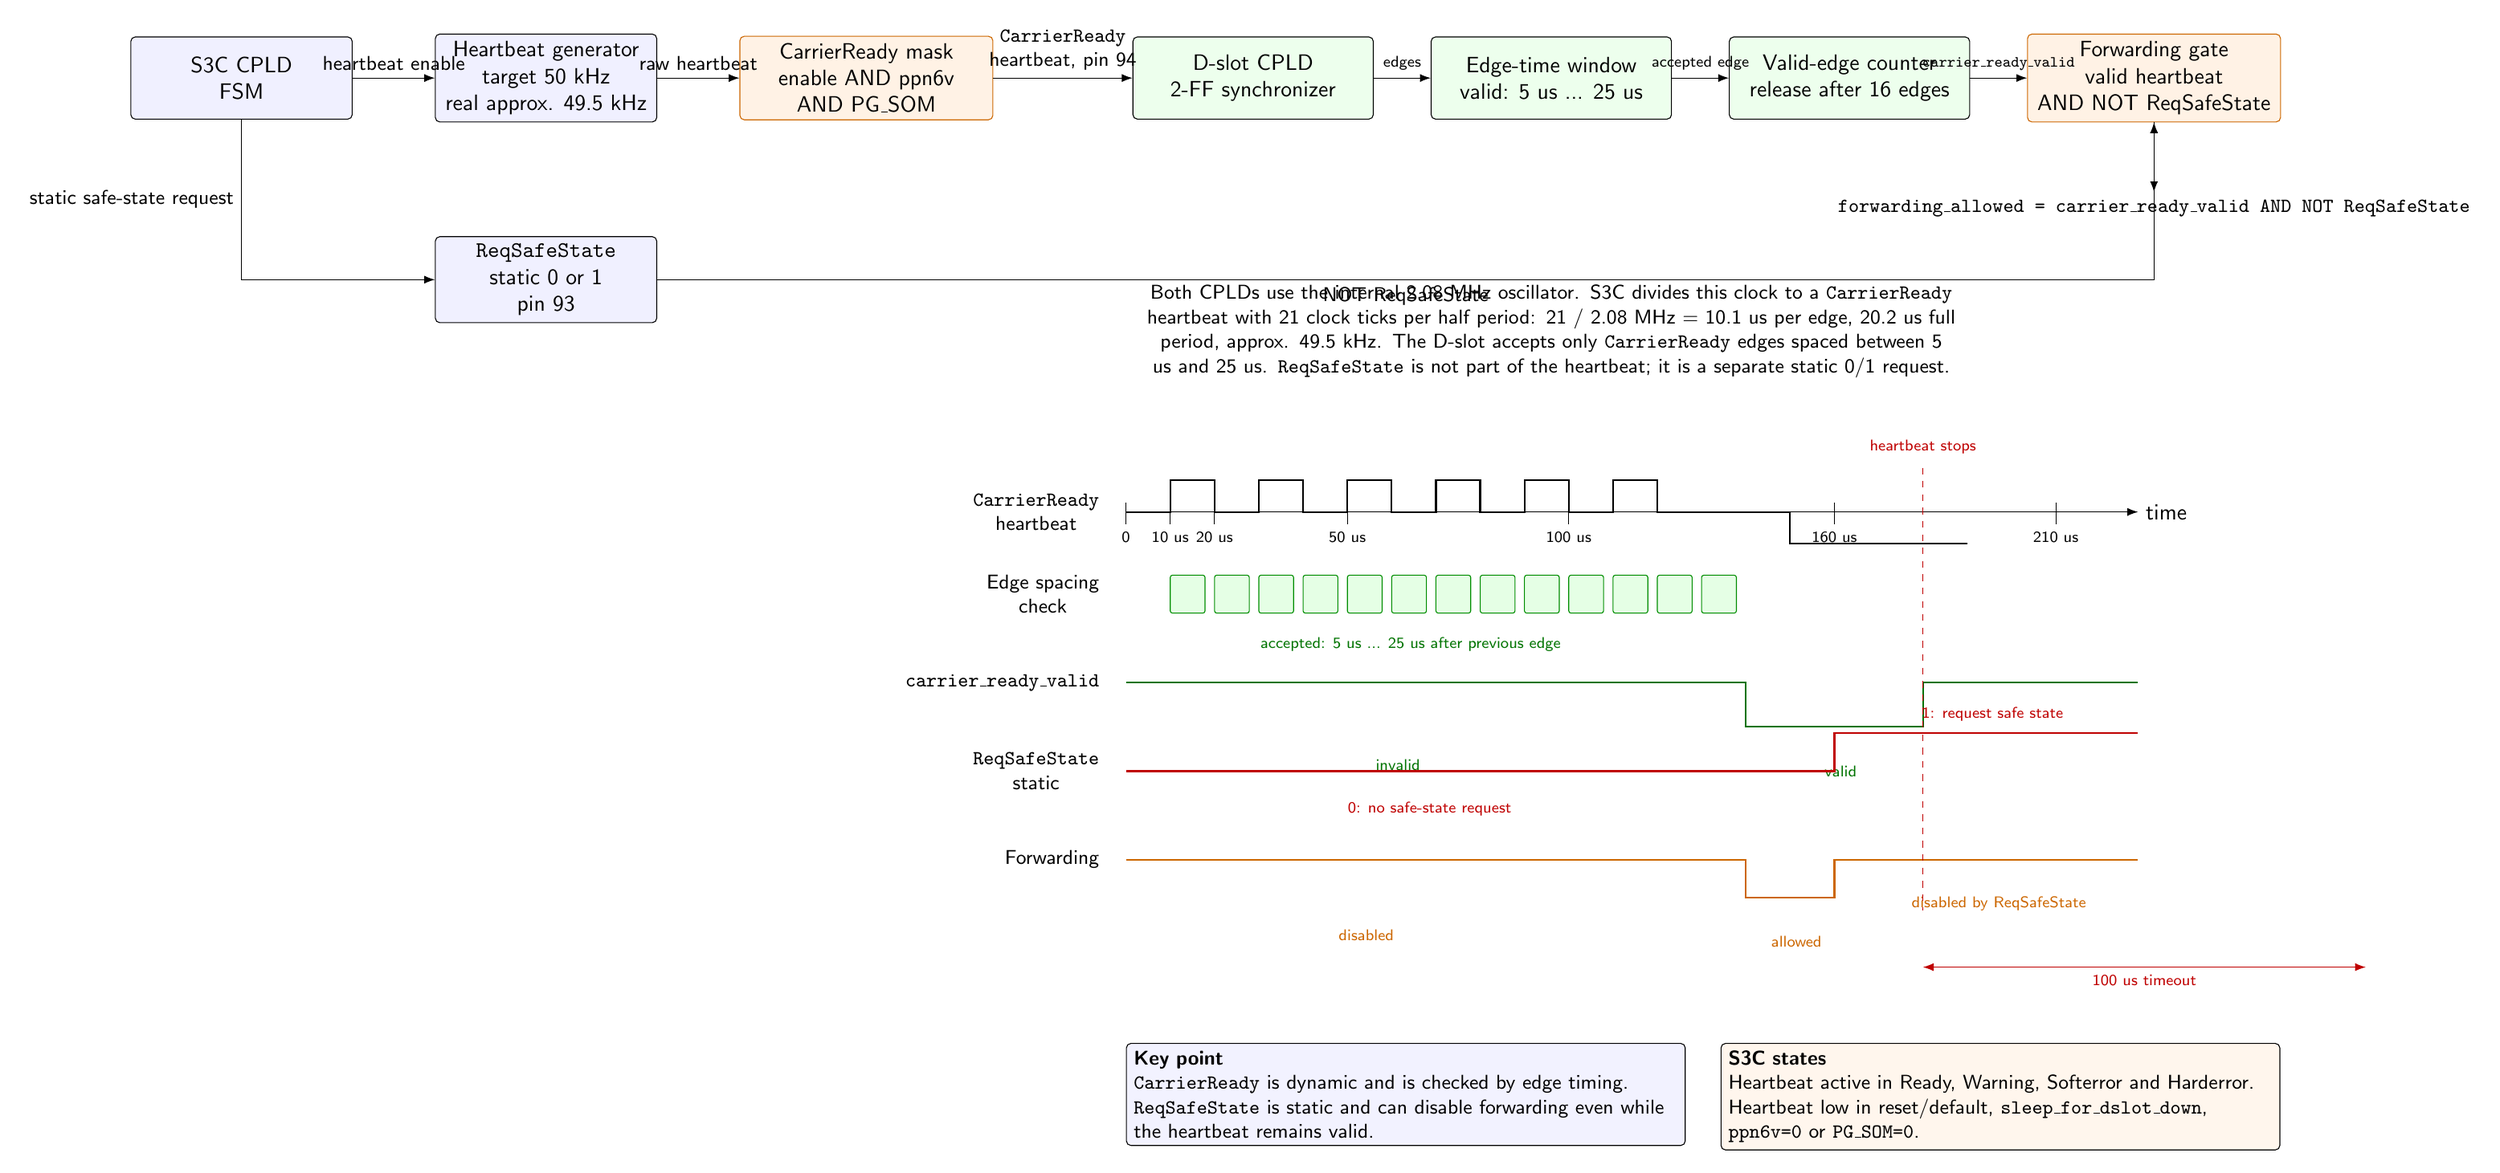
\begin{tikzpicture}[
  font=\sffamily,
  >=Latex,
  block/.style={draw, rounded corners=2pt, align=center, minimum height=13mm, minimum width=35mm, fill=blue!6},
  dblock/.style={draw, rounded corners=2pt, align=center, minimum height=13mm, minimum width=38mm, fill=green!7},
  gate/.style={draw=orange!80!black, fill=orange!10, rounded corners=2pt, align=center, minimum height=13mm, minimum width=40mm},
  note/.style={align=center, font=\sffamily\small},
  tinytext/.style={align=center, font=\sffamily\scriptsize},
  sig/.style={thick},
  good/.style={draw=green!55!black, fill=green!10, rounded corners=1pt}
]

% ---------------------------------------------------------------------------
% Handshake block diagram
% ---------------------------------------------------------------------------
\node[block] (s3cfsm) {S3C CPLD\\FSM};
\node[block, right=13mm of s3cfsm] (hbgen) {Heartbeat generator\\target 50 kHz\\real approx. 49.5 kHz};
\node[gate, right=13mm of hbgen] (hbgate) {CarrierReady mask\\enable AND ppn6v\\AND PG\_SOM};
\node[dblock, right=22mm of hbgate] (sync) {D-slot CPLD\\2-FF synchronizer};
\node[dblock, right=9mm of sync] (window) {Edge-time window\\valid: 5 us ... 25 us};
\node[dblock, right=9mm of window] (counter) {Valid-edge counter\\release after 16 edges};
\node[gate, right=9mm of counter] (forward) {Forwarding gate\\valid heartbeat\\AND NOT ReqSafeState};

\draw[->] (s3cfsm) -- node[above,note] {heartbeat enable} (hbgen);
\draw[->] (hbgen) -- node[above,note] {raw heartbeat} (hbgate);
\draw[->] (hbgate) -- node[above,note] {\texttt{CarrierReady}\\heartbeat, pin 94} (sync);
\draw[->] (sync) -- node[above,tinytext] {edges} (window);
\draw[->] (window) -- node[above,tinytext] {accepted edge} (counter);
\draw[->] (counter) -- node[above,tinytext] {\texttt{carrier\_ready\_valid}} (forward);

\node[block, below=18mm of hbgen] (reqsafe) {\texttt{ReqSafeState}\\static 0 or 1\\pin 93};
\draw[->] (s3cfsm.south) |- node[pos=.25,left,note] {static safe-state request} (reqsafe.west);
\draw[->] (reqsafe.east) -| node[pos=.25,below,note] {NOT ReqSafeState} (forward.south);

\node[note, below=11mm of forward] (out) {\texttt{forwarding\_allowed = carrier\_ready\_valid AND NOT ReqSafeState}};
\draw[->] (forward) -- (out);

\node[note, below=25mm of window, text width=132mm] (params) {
Both CPLDs use the internal 2.08 MHz oscillator. S3C divides this clock to a
\texttt{CarrierReady} heartbeat with 21 clock ticks per half period:
21 / 2.08 MHz = 10.1 us per edge, 20.2 us full period, approx. 49.5 kHz.
The D-slot accepts only \texttt{CarrierReady} edges spaced between 5 us and 25 us.
\texttt{ReqSafeState} is not part of the heartbeat; it is a separate static 0/1 request.
};

% ---------------------------------------------------------------------------
% Timing diagram, scaled in us
% scale: 1 us = 0.7 mm
% ---------------------------------------------------------------------------
\coordinate (t0) at ($(params.south west)+(0,-20mm)$);
\coordinate (tend) at ($(t0)+(160mm,0)$);
\draw[->] (t0) -- (tend) node[right] {time};

\node[note, anchor=east] at ($(t0)+(-3mm,0mm)$) {\texttt{CarrierReady}\\heartbeat};
\node[note, anchor=east] at ($(t0)+(-3mm,-13mm)$) {Edge spacing\\check};
\node[note, anchor=east] at ($(t0)+(-3mm,-27mm)$) {\texttt{carrier\_ready\_valid}};
\node[note, anchor=east] at ($(t0)+(-3mm,-41mm)$) {\texttt{ReqSafeState}\\static};
\node[note, anchor=east] at ($(t0)+(-3mm,-55mm)$) {Forwarding};

% Heartbeat waveform: 50 kHz target, one edge about every 10 us.
\draw[sig] ($(t0)+(0,0)$)
  -- ++(7mm,0) -- ++(0,5mm) -- ++(7mm,0) -- ++(0,-5mm)
  -- ++(7mm,0) -- ++(0,5mm) -- ++(7mm,0) -- ++(0,-5mm)
  -- ++(7mm,0) -- ++(0,5mm) -- ++(7mm,0) -- ++(0,-5mm)
  -- ++(7mm,0) -- ++(0,5mm) -- ++(7mm,0) -- ++(0,-5mm)
  -- ++(7mm,0) -- ++(0,5mm) -- ++(7mm,0) -- ++(0,-5mm)
  -- ++(7mm,0) -- ++(0,5mm) -- ++(7mm,0) -- ++(0,-5mm)
  -- ++(21mm,0)
  -- ++(0,-5mm) -- ++(28mm,0);

% Mark time ticks.
\foreach \x/\lab in {0/0,7/10 us,14/20 us,35/50 us,70/100 us,112/160 us,147/210 us} {
  \draw ($(t0)+(\x mm,1.5mm)$) -- ($(t0)+(\x mm,-2mm)$);
  \node[tinytext, anchor=north] at ($(t0)+(\x mm,-2mm)$) {\lab};
}

% Edge spacing accepted windows.
\foreach \x in {7,14,21,28,35,42,49,56,63,70,77,84,91} {
  \draw[good] ($(t0)+(\x mm,-16mm)$) rectangle ++(5.5mm,6mm);
}
\node[tinytext, green!45!black] at ($(t0)+(45mm,-21mm)$) {accepted: 5 us ... 25 us after previous edge};

% Valid waveform: invalid initially, valid after many valid edges, timeout later.
\draw[sig, green!45!black] ($(t0)+(0,-27mm)$) -- ++(98mm,0)
  -- ++(0,-7mm) -- ++(28mm,0)
  -- ++(0,7mm) -- ++(34mm,0);
\node[tinytext, green!45!black] at ($(t0)+(43mm,-40mm)$) {invalid};
\node[tinytext, green!45!black] at ($(t0)+(113mm,-41mm)$) {valid};

% ReqSafeState static request: low, then high while heartbeat may still run.
\draw[sig, red!75!black] ($(t0)+(0,-41mm)$) -- ++(112mm,0)
  -- ++(0,6mm) -- ++(48mm,0);
\node[tinytext, red!75!black] at ($(t0)+(48mm,-47mm)$) {0: no safe-state request};
\node[tinytext, red!75!black] at ($(t0)+(137mm,-32mm)$) {1: request safe state};

% Forwarding: only when heartbeat valid and ReqSafeState low.
\draw[sig, orange!80!black] ($(t0)+(0,-55mm)$) -- ++(98mm,0)
  -- ++(0,-6mm) -- ++(14mm,0)
  -- ++(0,6mm) -- ++(48mm,0);
\node[tinytext, orange!80!black] at ($(t0)+(38mm,-67mm)$) {disabled};
\node[tinytext, orange!80!black] at ($(t0)+(106mm,-68mm)$) {allowed};
\node[tinytext, orange!80!black] at ($(t0)+(138mm,-62mm)$) {disabled by ReqSafeState};

% Timeout zone: heartbeat stops and 100 us timeout invalidates heartbeat.
\draw[dashed, red!75!black] ($(t0)+(126mm,7mm)$) -- ($(t0)+(126mm,-63mm)$);
\node[tinytext, red!75!black, anchor=south] at ($(t0)+(126mm,8mm)$) {heartbeat stops};
\draw[<->, red!75!black] ($(t0)+(126mm,-72mm)$) -- node[below,tinytext] {100 us timeout} ($(t0)+(196mm,-72mm)$);

\node[draw, rounded corners=2pt, fill=blue!5, align=left, font=\sffamily\small, anchor=north west, text width=86mm]
  at ($(t0)+(0mm,-84mm)$) {
  \textbf{Key point}\\
  \texttt{CarrierReady} is dynamic and is checked by edge timing.\\
  \texttt{ReqSafeState} is static and can disable forwarding even while the heartbeat remains valid.
  };

\node[draw, rounded corners=2pt, fill=orange!7, align=left, font=\sffamily\small, anchor=north west, text width=86mm]
  at ($(t0)+(94mm,-84mm)$) {
  \textbf{S3C states}\\
  Heartbeat active in Ready, Warning, Softerror and Harderror.\\
  Heartbeat low in reset/default, \texttt{sleep\_for\_dslot\_down}, \texttt{ppn6v=0} or \texttt{PG\_SOM=0}.
  };

\end{tikzpicture}
\end{document}
